% ------------------------------------------------------------------------ %
% !TEX encoding = UTF-8 Unicode
% !TEX TS-program = pdflatex
% !TEX root = ../Tesi.tex
% !TEX spellcheck = it-IT
% ------------------------------------------------------------------------ %
%
% ------------------------------------------------------------------------ %
% 	STATO DELL'ARTE
% ------------------------------------------------------------------------ %
%
\chapter{State of the Art}
%
\label{cap:statoarte}
%
% ------------------------------------------------------------------------ %
%
\section{Android OS} \label{androidos}
\par As already mentioned in \ref{motivation}, the Android operating system is an open source OS developed by Google based on Linux kernel, that can be installed on many different kind of devices.\\
In this section i want to give to the reader the basic knowledge of the Android framework to understand why and how the operating system works.
\subsection{Brief History}  
\par
The Android era officially began on October 22nd, 2008, when the \textit{T-Mobile G1} launched in the United States \cite{verge2011android}.\\
At that moment the company of mountain view, Google, felt the need to create a new operating system which was able to be installed on most modern mobile phones of the time. To meet this need the Google engineers created an OS that was based on the Linux kernel, lightweight enough and ease to be used with simple hand gestures by touching the screen of the phone.\\

\begin{figure}[h]
	\centering
	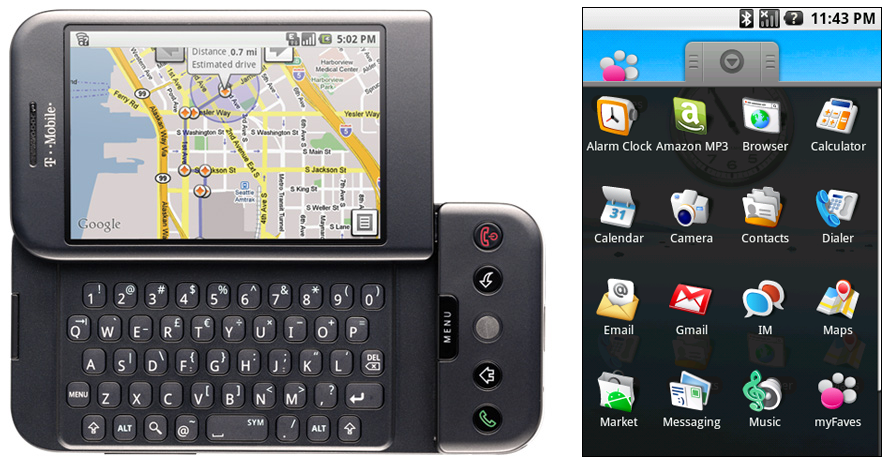
\includegraphics[width=0.8\textwidth]{T-MobileG1Android1menu}
	\caption{The T-Mobile G1 and the Android 1.0 menù}
	\label{2.1:The T-Mobile G1 and the Android 1.0 menù}
\end{figure}

The main characteristic of the OS were and are also now:
\begin{itemize}
	\item The pull-down notification window.
	\item Home screen widgets.
	\item The Android Market.
	\item Google services integration (eg. Gmail).
	\item Wireless connection technologies (eg Wi-Fi and Bluetooth)
\end{itemize}
The success of the first version of the brand new mobile operating system and the open source philosophy guaranteed the fast spread of the Android devices all over the world. In few years Google improved and released many version of the OS and with the help of the market growth Android has become a complete os. 
In the table below there is a brief description of the various distribution of the Android OS at the time of writing of this document.\\
\begin{table}[h]
	%
	\caption{Android versions}
	%
	\label{tab:vers}
	%
	\centering
	%
	\begin{tabular}{llll}
		%
		\toprule
		%
		\textbf{Name} & \textbf{Version}  & \textbf{Release Date} & \textbf{API Level}\\
		%
		\midrule
		%
		Alpha &	1.0 & September 23, 2008 & 1 \\
		Beta & 1.1 & February 9, 2009 & 2 \\
		Cupcake & 1.5 & April 27, 2009 & 3 \\
		Donut &	1.6 & September 15, 2009 & 4 \\
		Eclair & 2.0 – 2.1 & October 26, 2009 & 5–7 \\
		Froyo & 2.2 – 2.2.3 & May 20, 2010 & 8 \\
		Gingerbread & 2.3 – 2.3.7 & December 6, 2010 & 9–10 \\	
		Honeycomb & 3.0 – 3.2.6 & February 22, 2011 & 11–13 \\
		Ice Cream Sandwich & 4.0 – 4.0.4 & October 18, 2011 & 14–15 \\
		Jelly Bean & 4.1 – 4.3.1 & July 9, 2012 & 16–18 \\
		KitKat & 4.4 – 4.4.4 & October 31, 2013 & 19 \\
		Lollipop & 5.0 – 5.1.1 & November 12, 2014 & 21–22 \\
		Marshmallow & 6.0 – 6.0.1 & October 5, 2015 & 23 \\
		Nougat & 7.0 – 7.1.1 & August 22, 2016 & 24–25 \\
		%
		\bottomrule
		%
	\end{tabular}
	%
\end{table}
 As we can see in \tablename~\ref{tab:vers} there are, currently, 25 level of the Android \textit{API} (Application programming interface
 ) which developers can use to build Android applications. In particular various API levels introduce innovations in the OS but, applications developed using an higher \textit{API level} can not be executed in a device running lower versions of the operating system. This is a second major limitations for the \textit{"Android ecosystem"}, moreover as mentioned before, the Android OS is released under an open source license, which is great for the developer, but which prevents Google to provide updates, in a centralized way, to all devices. For this reason there are currently many active devices running different versions of the mobile OS, as we can check in \tablename~\ref{tab:chart}, which shows, in percentage, the fragmentations of active machines running Android OS.\\
 \begin{table}[h]
 	%
 	\caption{Android OS versions fragmentation}
 	%
 	\label{tab:chart}
 	%
 	
 	%
 	\begin{minipage}{0.5\textwidth}
 		\centering
 		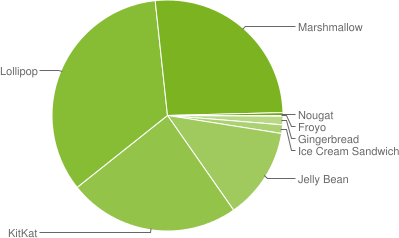
\includegraphics[width=0.9\textwidth]{androidversionchart}
 		 \captionof{figure}{Android OS fragmentation chart}
 		\label{2.2:Android fragmentation chart}
 		
 	\end{minipage}
 ~\hfill~
 \begin{minipage}{0.5 \textwidth}
 	\centering
 	\begin{tabular}{lll}
 		%
 		\toprule
 		%
 		\textbf{Version}  & \textbf{API Level} & \textbf{Distribution}\\
 		%
 		\midrule
 		%
 		2.2 & 8 & 0.1\% \\
 		2.3.3 - 2.3.7 & 10 & 1.2\% \\
 		4.0.3 - 4.0.4 & 15 & 1.2\% \\
 		4.1.x & 16 & 4.5\% \\
 		4.2.x & 17 & 6.4\% \\
 		4.3 & 18 & 1.9\% \\
 		4.4 & 19 & 24.0\% \\
 		5.0 & 21 & 10.8\% \\
 		5.1 & 22 & 23.2\% \\
 		6.0 & 23 & 26.3\% \\
 		7.0 & 24 & 0.4\% \\
 		%
 		\bottomrule
 		%
 	\end{tabular}
\end{minipage}
 	%
 \end{table}
Data in \tablename~\ref{tab:chart} were collected during a 7-day period ending on December 5, 2016, by Google. Any versions with less than 0.1\% distribution are not shown \cite{devandroiddash}.
\subsection{Structure}
\par
Android is an operating system based on the Linux kernel. The project responsible for developing the Android system is called the \textit{Android Open Source Project (AOSP)} and it lead by Google.
\begin{figure}[h]
	\centering
	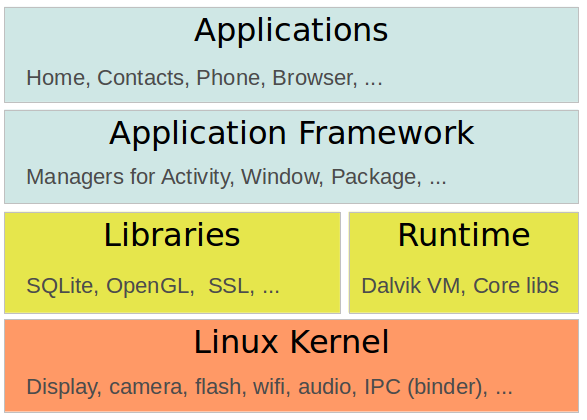
\includegraphics[width=0.8\textwidth]{oslevels}
	\caption{Android OS 4 layers}
	\label{fig:2.3}
\end{figure}

The OS can be divided into the four layers as depicted the \figurename~\ref{fig:2.3}. An Android application developer typically works with the two layers on top to create new Android applications \cite{vogel2016android}.

\paragraph{Linux Kernel} is the most flexible operating system that has ever been created. It can be tuned for a wide range of different systems, running on everything from a radio-controlled model helicopter, to a cell phone, to the majority of the largest supercomputers in the world \cite{hartman2006linux}. This is in practice the communication layer for the underlying hardware.
\paragraph{Runtime and Libraries} \par Runtime is the term used in computer science to designate the software that provides the services necessary for the execution of a program.There are two different \textit{"runtime systems"} which can work with the Android OS:
\begin{itemize}
	\item \textit{Dalvik VM} is an optimized version for low memory devices of the \textit{Java Virtual Machine (JVM)} used in Android 4.4 and earlier version. It is stack based and it works by converting using a \textit{just-in-time (JIT)}, each time an application is executed, Android's \textit{bytecode} into machine code.
	\item \textit{ART (Android Runtime)} introduced with Android 4.4 KitKat. This runtime uses an \textit{AOT (Ahead-of-Time)} approach, with which code is compiled during the installation of an application and then is ready to be executed.
\end{itemize}
\par Standard Android libraries are for many common framework functions, like, graphic rendering, data storage, web browsing. \cite{vogel2016android}. This layer contains also standard \textit{java libraries}.
\paragraph{Application Framework}\label{appframework} is the layer that contains the Android components for the application such as activities, fragments, services and so on. 
\paragraph{Applications} are pieces of software written in \textit{java code} running on top the other layers.

\subsection{Application Framework}
In this section I want to give some details of the application composition and work flow to better understand the subsequent sections in which I will describe the given problem and the proposed solution.\\
As briefly described in \ref{appframework} the Android application framework \textit{("AppFramework")} is the core of the Android \textit{development API}. It contains useful and needed components to build native apps.\\
The main components with which each application is composed are:

\paragraph{Intents} are objects that initiate actions from other app components, either within the same program \textit{(explicit intents)} or through another piece of software on the device \textit{(implicit intents)}.
Acconrding to the official Google's Android for developer documentation, an Intent is a sort of messaging object which can be used to request an action from another application component (eg. activities). There are three fundamental use cases:
\begin{itemize}
	\item Starting an activity: we will see that activities represents a single screen in Android applications, intents allow to start activities by describing them and carrying any necessary data.
	\item Starting a service: I will explain later in deeper details that services are component which performs operations in background. As for the activities, services are initialized through intent and in the same way they describe the service to start and carries any necessary data.
	\item Delivering a broadcast: broadcast is a message that any app can receive. The system delivers various broadcasts for system events, such as when the system boots up or the device starts charging.
\end{itemize}

As already mentioned there are mainly two categories of intents:
\begin{itemize}
	\item explicit intents, used when it is needed to start component within the same application. As the name implies explicit intents call components by using by name (the full \textit{class object} name), for example, it is possible to start a new activity in response to a user action or start a service to download a file in the background.
	\item implicit intents do not name a specific component, but instead declare a general action to perform, which allows a component from another app to handle it. For example, if you want to show the user a location on a map, you can use an implicit intent to request that another capable app show a specified location on a map \cite{devandroidintent}.
\end{itemize}

\begin{figure}[h]
	\centering
	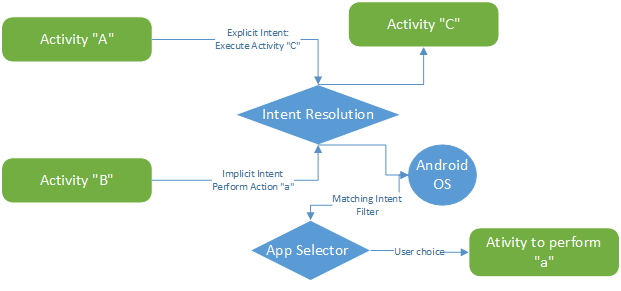
\includegraphics[width=0.9\textwidth]{intentresolution}
	\caption{Intent resolution mechanism}
	\label{fig:2.4}
\end{figure}

The \figurename~\ref{fig:2.4} explains well how an intent is resolved by the OS whether it is implicit or explicit. When an implicit intent needs to be resolved, the OS searches applications which can handle it by means of \textit{intent filters}.A Intent filter specifies the types of intents that an activity, service, or broadcast receiver can respond to. The Android System searches all apps for an intent filter that matches the intent to be resolved. When a match is found, the system starts the matching component, or, if there are more than one, let the user select the preferred action to be performed.

\paragraph{Activities} are one of the fundamental building blocks of apps on the Android platform. They serve as the entry point for a user's interaction with an app, and are also central to how a user navigates within an app. \cite{devandroidactivity}

\paragraph{Services}

\subsection{Connectivity}

\subsection{Permissions \& Security}

 
\section{Distributed System} \label{distsys}
\subsection{Definition}

\subsection{Examples} \label{distex}


\section{Liquid Computation}
\subsection{Definition}
\par 




I have only quickly listed some features and possible issues of my source, to have a complete idea it is possible to read all the proposed solutions and ideas in \cite{guinard2011web}.
%
% ------------------------------------------------------------------------ %6